
\begin{slide}[Replace]{The counterexample}

\centerline{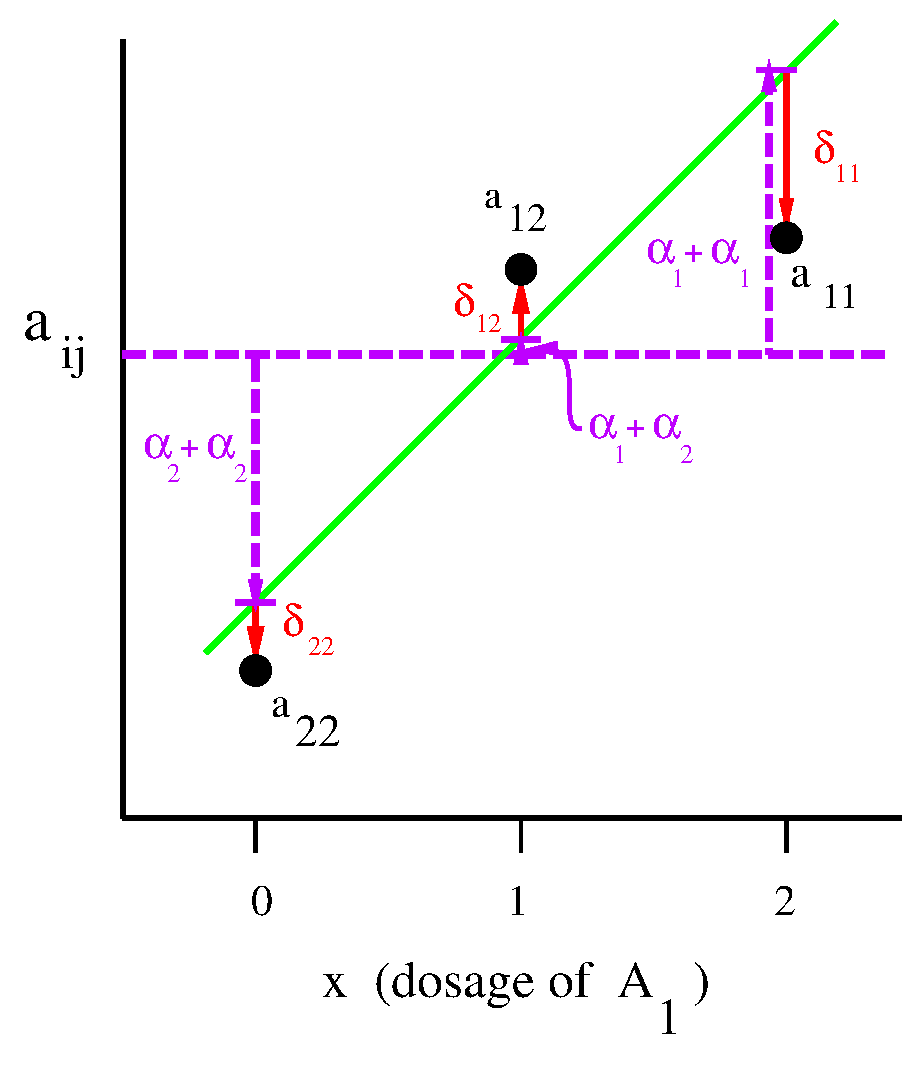
\includegraphics[width=2.5in]{fig9-3.ydraw}}
\bigskip

The long branches have probabilities of change $\ \mathsf{p}$, the short
branches have probabilities of change $\ \mathsf{q}$.  This is the canonical
case of ``long branch attraction''.

\end{slide}

\begin{slide}[Replace]{Pattern probabilities}

If tip pattern is 1100, and internal nodes are 1, 1 the probability is
\[
\mathsf{\frac{1}{2}(1-p)(1-q)(1-q)pq}
\]

and in general summing over all four possibilities:
\[
\begin{array}{c c l}
\mathsf{P_{1100}} & \mathsf{=} &  \mathsf{\frac{1}{2}\left((1-p)(1-q)^2pq\ +\ (1-p)^2(1-q)^2q\right.}\\
& & \\
  & & \mathsf{\left.+\ p^2q^3\ +\ pq(1-p)(1-q)^2\right)}
\end{array}
\]

\end{slide}

\begin{slide}[Replace]{Pattern probabilities}

\noindent
\[
\begin{array}{c c l}
\mathsf{P_{xxyy}} &  \mathsf{=} &  \mathsf{(1-p)(1-q)[q(1-q)(1-p)\ +\ q(1-q)p]}\\\
& & \\
& &  \mathsf{+\  pq[(1-q)^2(1-p)\ +\ q^2p]} \\
& & \\
& & \\
\mathsf{P_{xyxy}} & \mathsf{=} & \mathsf{(1-p)q[q(1-q)p+q(1-q)(1-p)]}\\
& & \\
 & & \mathsf{+\ p(1-q)[p(1-q)^2\ +\ (1-p)q^2]} \\
& & \\
& & \\
\mathsf{P_{xyyx}} & \mathsf{=} &  \mathsf{(1-p)q[(1-p)q^2+p(1-q)^2]}\\
& & \\
 & &\mathsf{+\ p(1-q)[q(1-q)p +\ q(1-q)(1-p)]}
\end{array}
\]
 
\end{slide}

\begin{slide}[Replace]{Taking differences}

\noindent
\[
\mathsf{P_{xyxy} - P_{xyyx} \ =\ (1-2q)\;\left[q^2(1-p)^2\ +\ (1-q)^2p^2\right]}
\]
\medskip

Which is always positive as long as $\mathsf{~q < 1/2~}$ and either
$\mathsf{~p~}$ or $\mathsf{~q~}$ is positive.  Thus $\mathsf{~P_{xyxy} >
P_{xyyx}~}$ so we don't need to concern ourselves with $\ \mathsf{P_{xyyx}}$.
\bigskip

To have $\mathsf{P_{xxyy}}$ be the largest of the three, we only need to
know that
\[
\mathsf{P_{xxyy} - P_{xyxy}\ >\ 0}
\]

and after a struggle that turns out to require
\[
\mathsf{(1-2q)\;\left[q(1-q)\ -\ p^2 \right]\ >\ 0}
\]

which (provided $\mathsf{q < 1/2}$) is true if and only if
\[
\mathsf{q(1-q)\  >\  p^2}
\]

\end{slide}

\begin{slide}[Replace]{Pattern frequencies win out}
\bigskip

\centerline{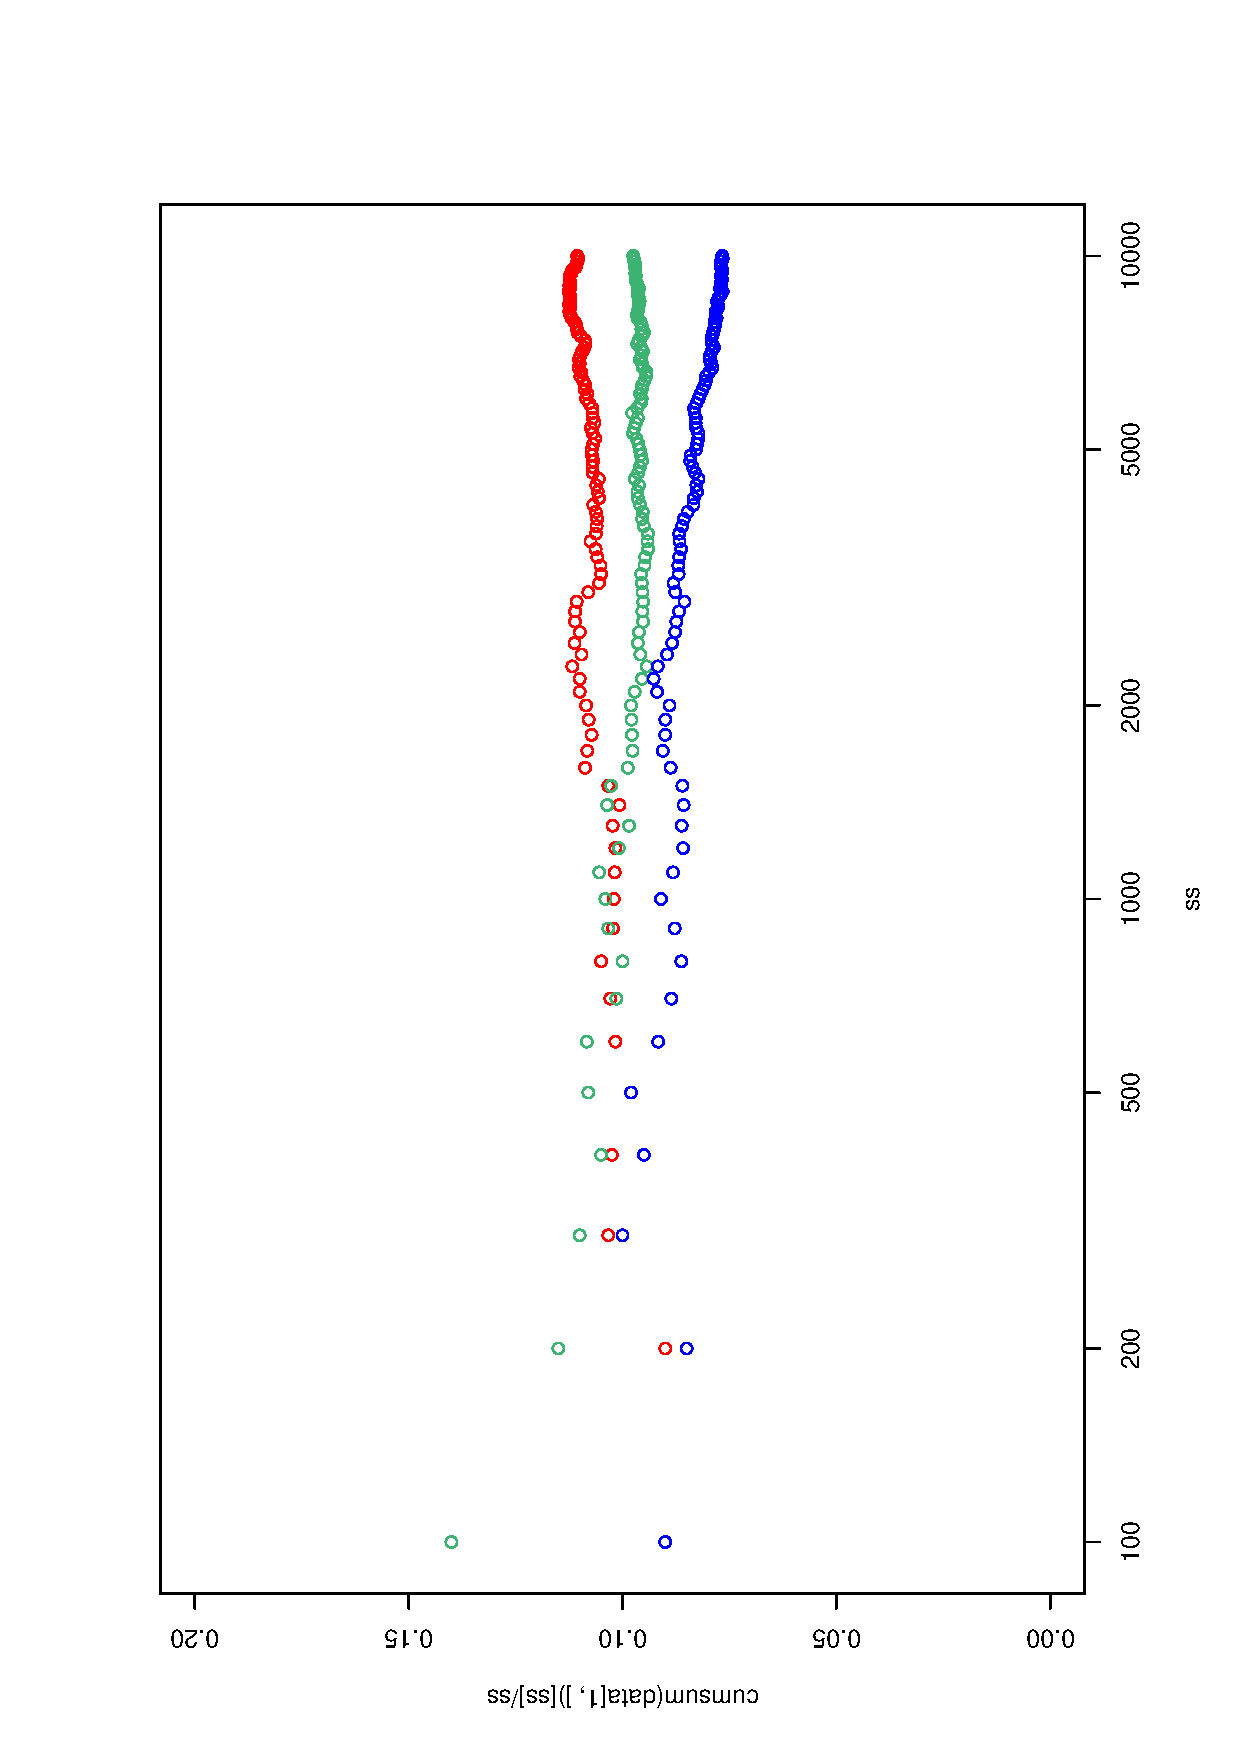
\includegraphics[width=4.0in]{largenumbers.idraw}}

\end{slide}

\begin{slide}[Replace]{Conditions for inconsistency}

\centerline{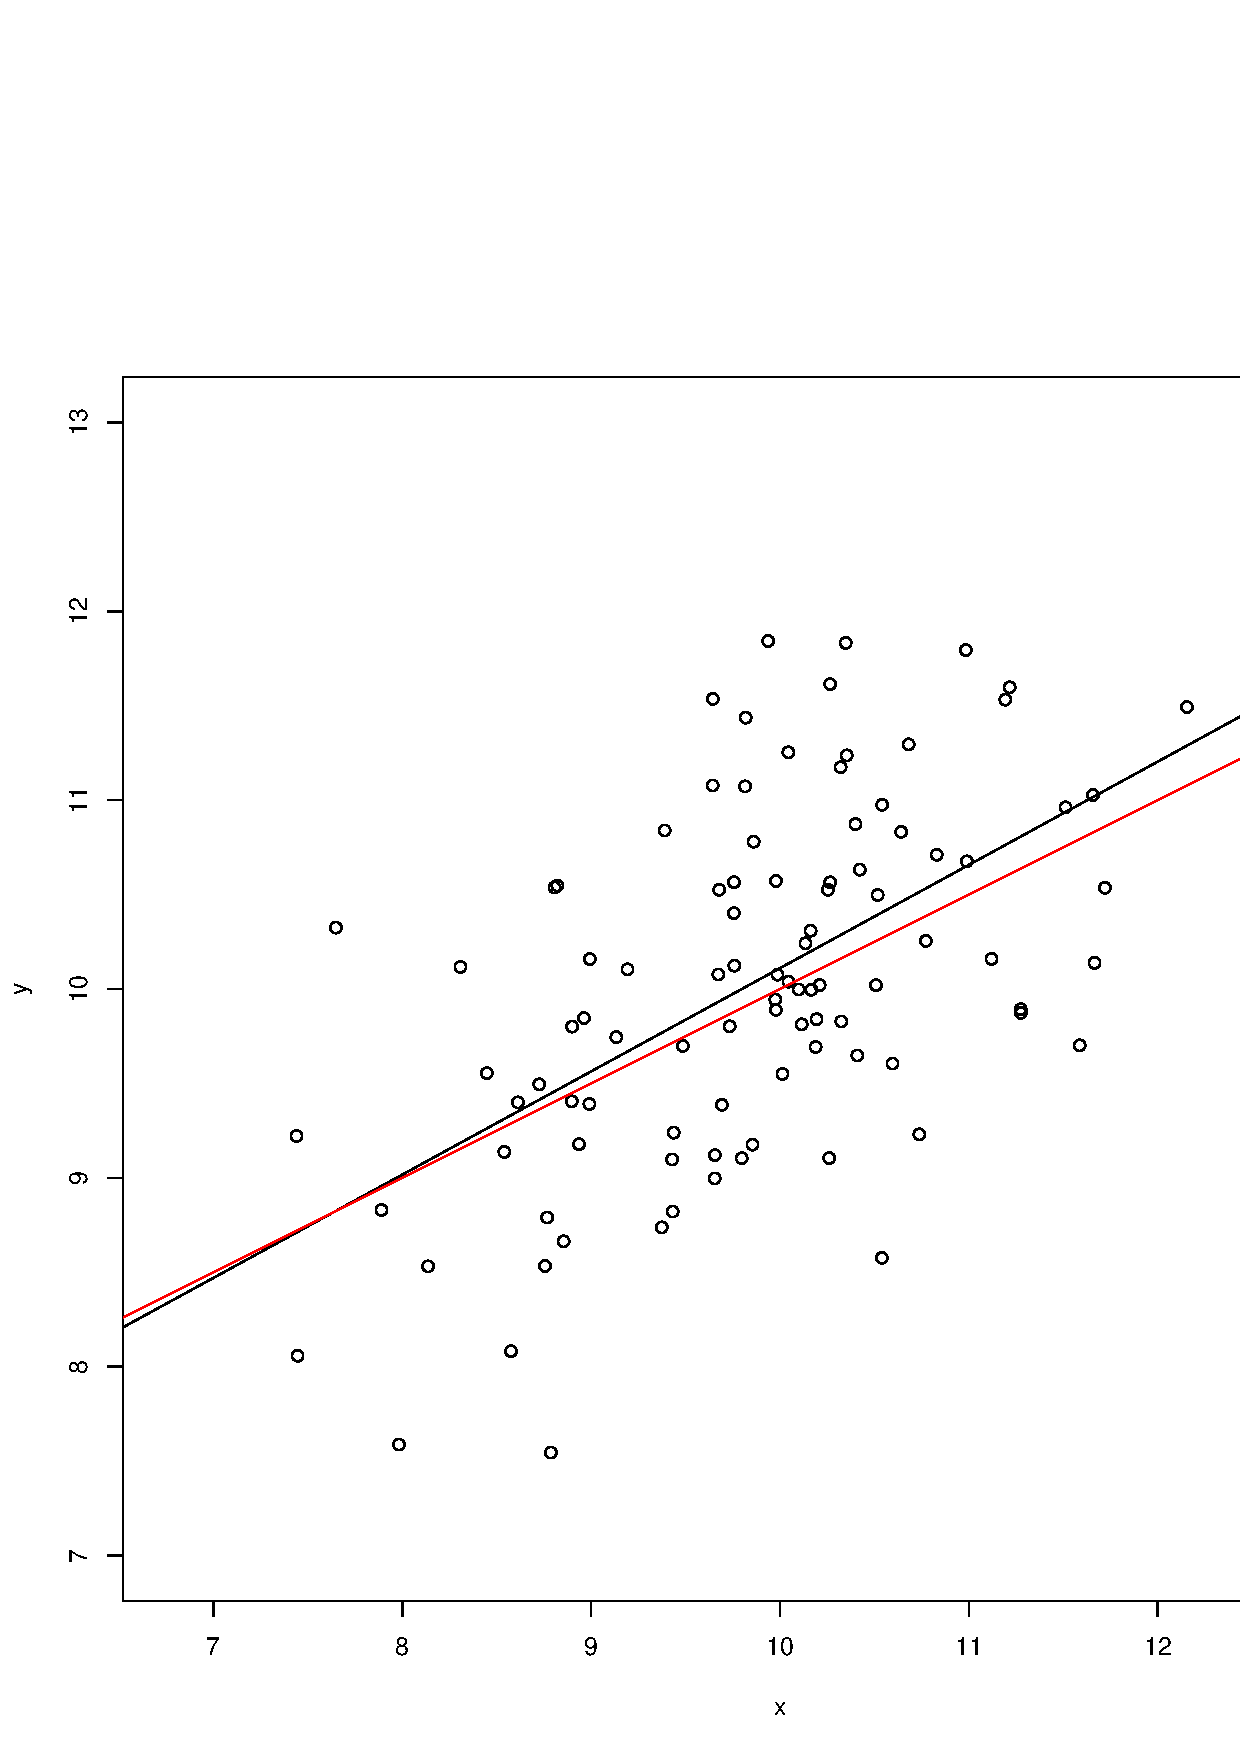
\includegraphics[width=3.2in]{fig9-5.ydraw}}

\end{slide}

\begin{slide}[Replace]{Example for patterns with DNA}

\centerline{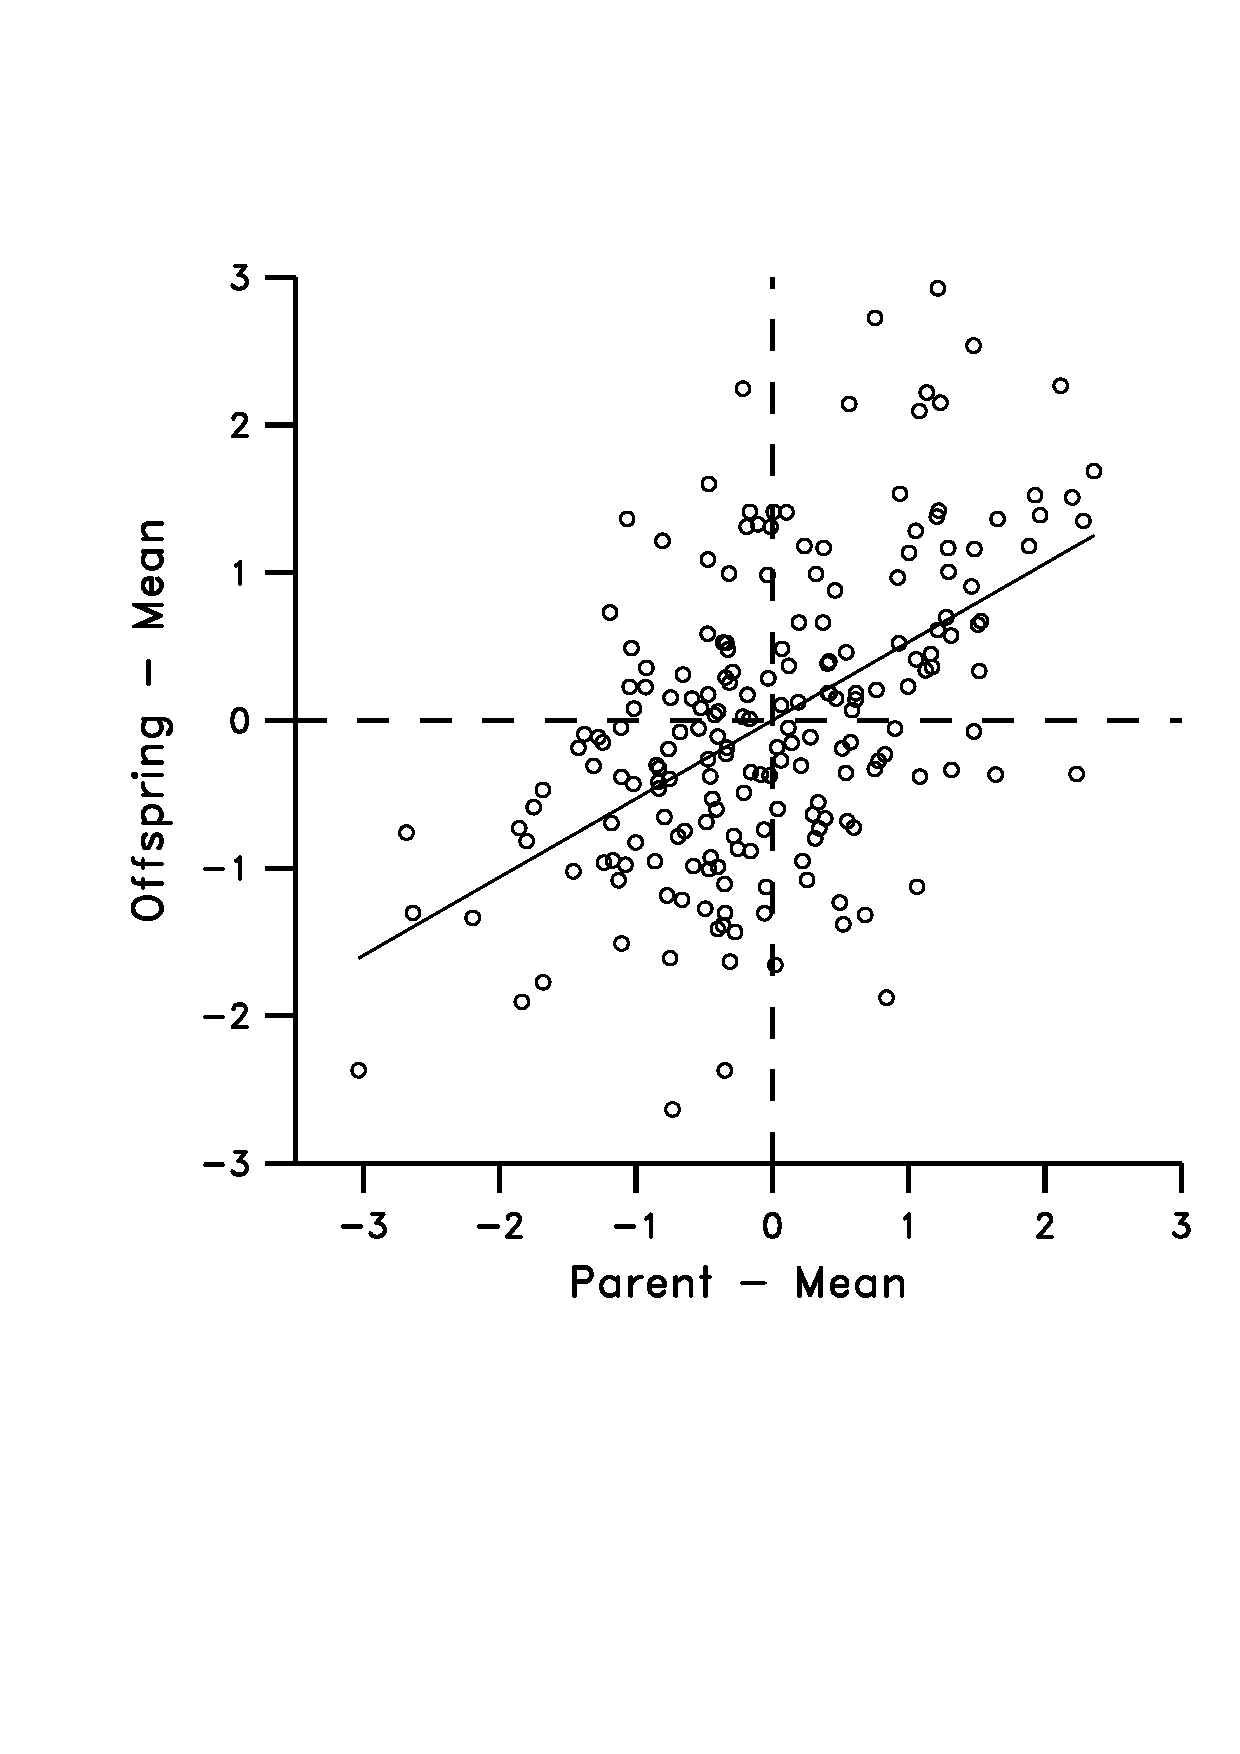
\includegraphics[width=2.5in]{fig9-6.ydraw}}

